\documentclass[12pt]{article}

% Packages
\usepackage[margin=1in]{geometry}
\usepackage{amsmath, amsthm, amssymb, physics, graphicx, pdfpages}

% Problem Box
\setlength{\fboxsep}{4pt}
\newsavebox{\savefullbox}
\newenvironment{fullbox}{\begin{lrbox}{\savefullbox}\begin{minipage}{\dimexpr\textwidth-2\fboxsep\relax}}{\end{minipage}\end{lrbox}\begin{center}\framebox[\textwidth]{\usebox{\savefullbox}}\end{center}}
\newenvironment{pbox}[1][]{\begin{fullbox}\ifx#1\empty\else\paragraph{#1}\fi}{\end{fullbox}}

% Options
\allowdisplaybreaks
\addtolength{\jot}{1em}
\theoremstyle{definition}
\setlength{\parindent}{0pt}
\setlength{\parskip}{6pt}

% Default Commands
\newtheorem{proposition}{Proposition}
\newtheorem{lemma}{Lemma}
\newcommand{\ds}{\displaystyle}
\newcommand{\isp}[1]{\quad\text{#1}\quad}
\newcommand{\N}{\mathbb{N}}
\newcommand{\Z}{\mathbb{Z}}
\newcommand{\Q}{\mathbb{Q}}
\newcommand{\R}{\mathbb{R}}
\newcommand{\C}{\mathbb{C}}
\newcommand{\eps}{\varepsilon}
\renewcommand{\phi}{\varphi}
\renewcommand{\emptyset}{\varnothing}

% Extra Commands


% Document Info
\title{\vspace{-0.5in}Assignment 6 \\
    \large GEOG 191
}
\author{Harry Coleman}
\date{February 17, 2021}

% Begin Document
\begin{document}
\maketitle

\section*{2}
Since there is more supply than demand, we add a dummy source, with objective coefficients of zero.

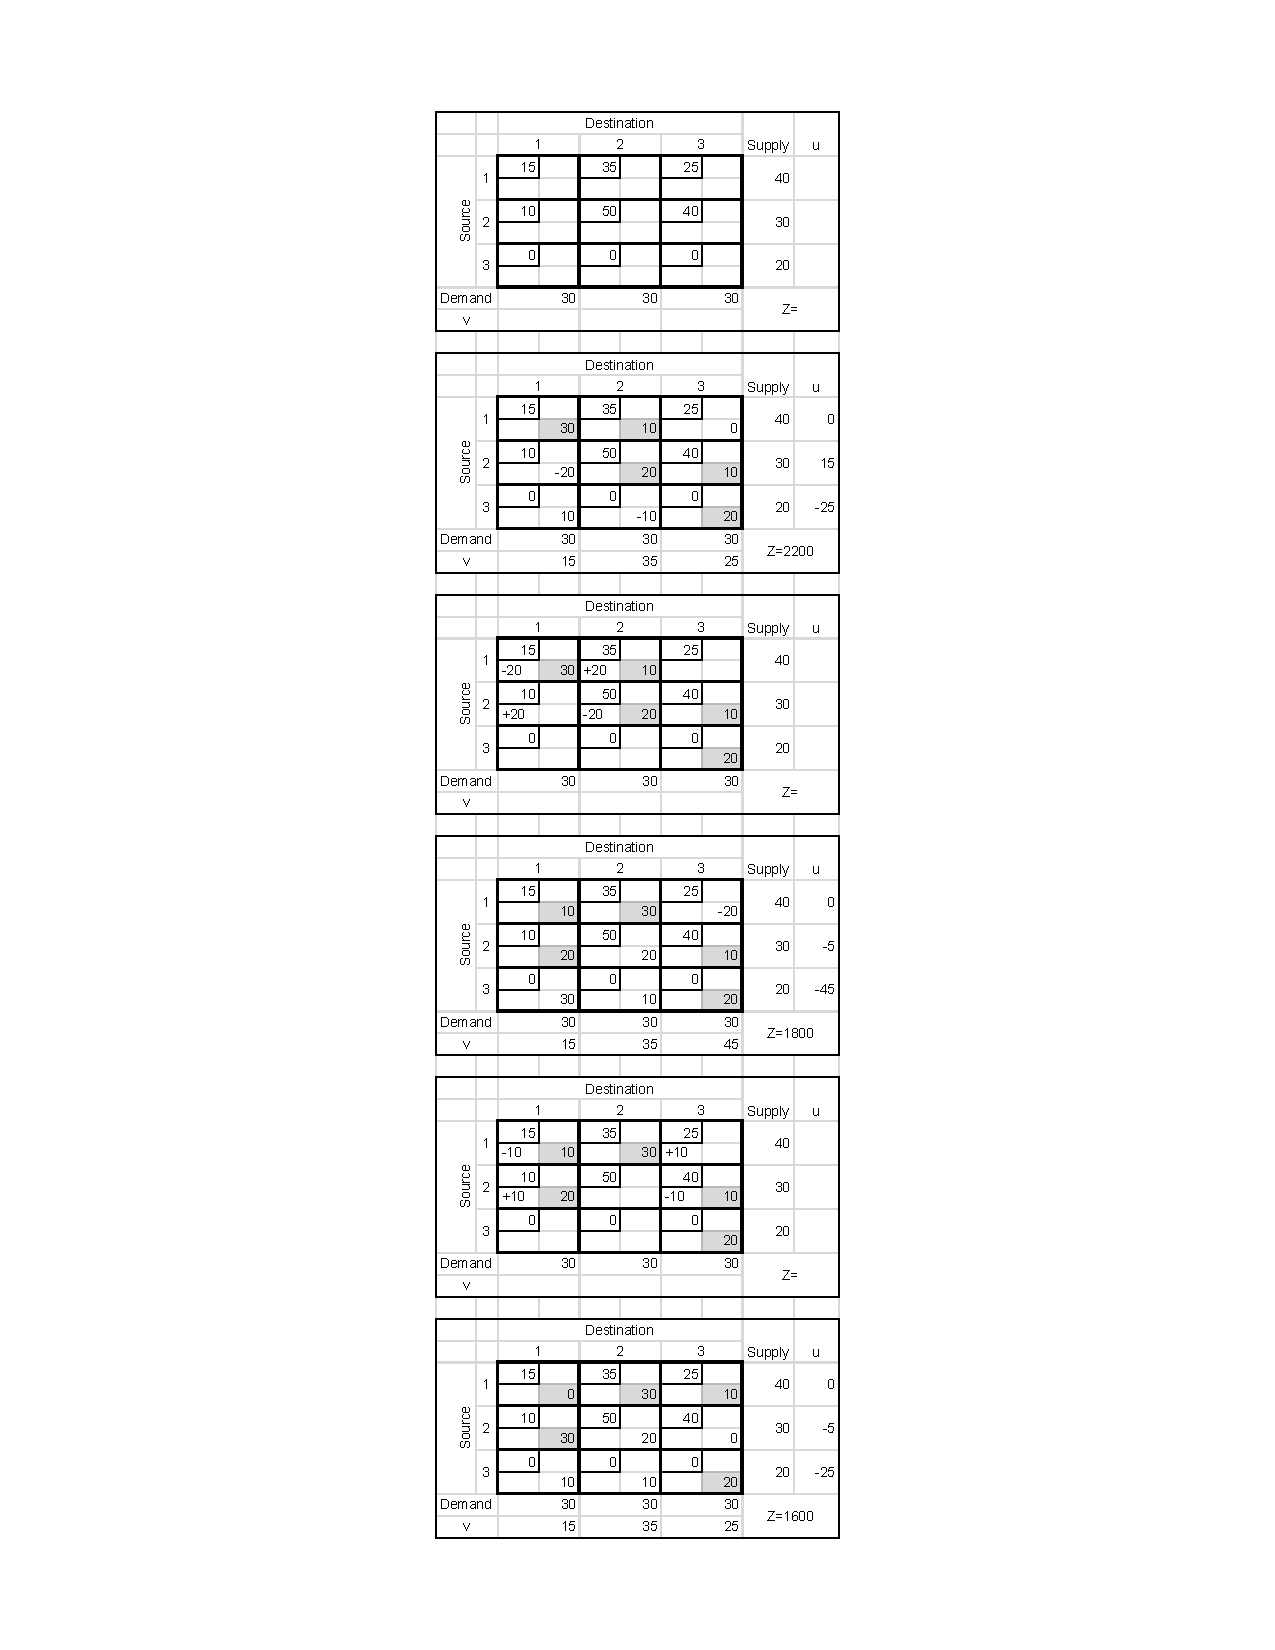
\includepdf[pages=-,pagecommand={},width=8in]{sheet1.pdf}

Discarding the dummy variables, we obtain an optimal solution with objective $Z = 1600$ and decision variable values
\[
    X = \mqty[0 & 30 & 10 \\ 30 & 0 & 10].
\]

\newpage
\section*{4}
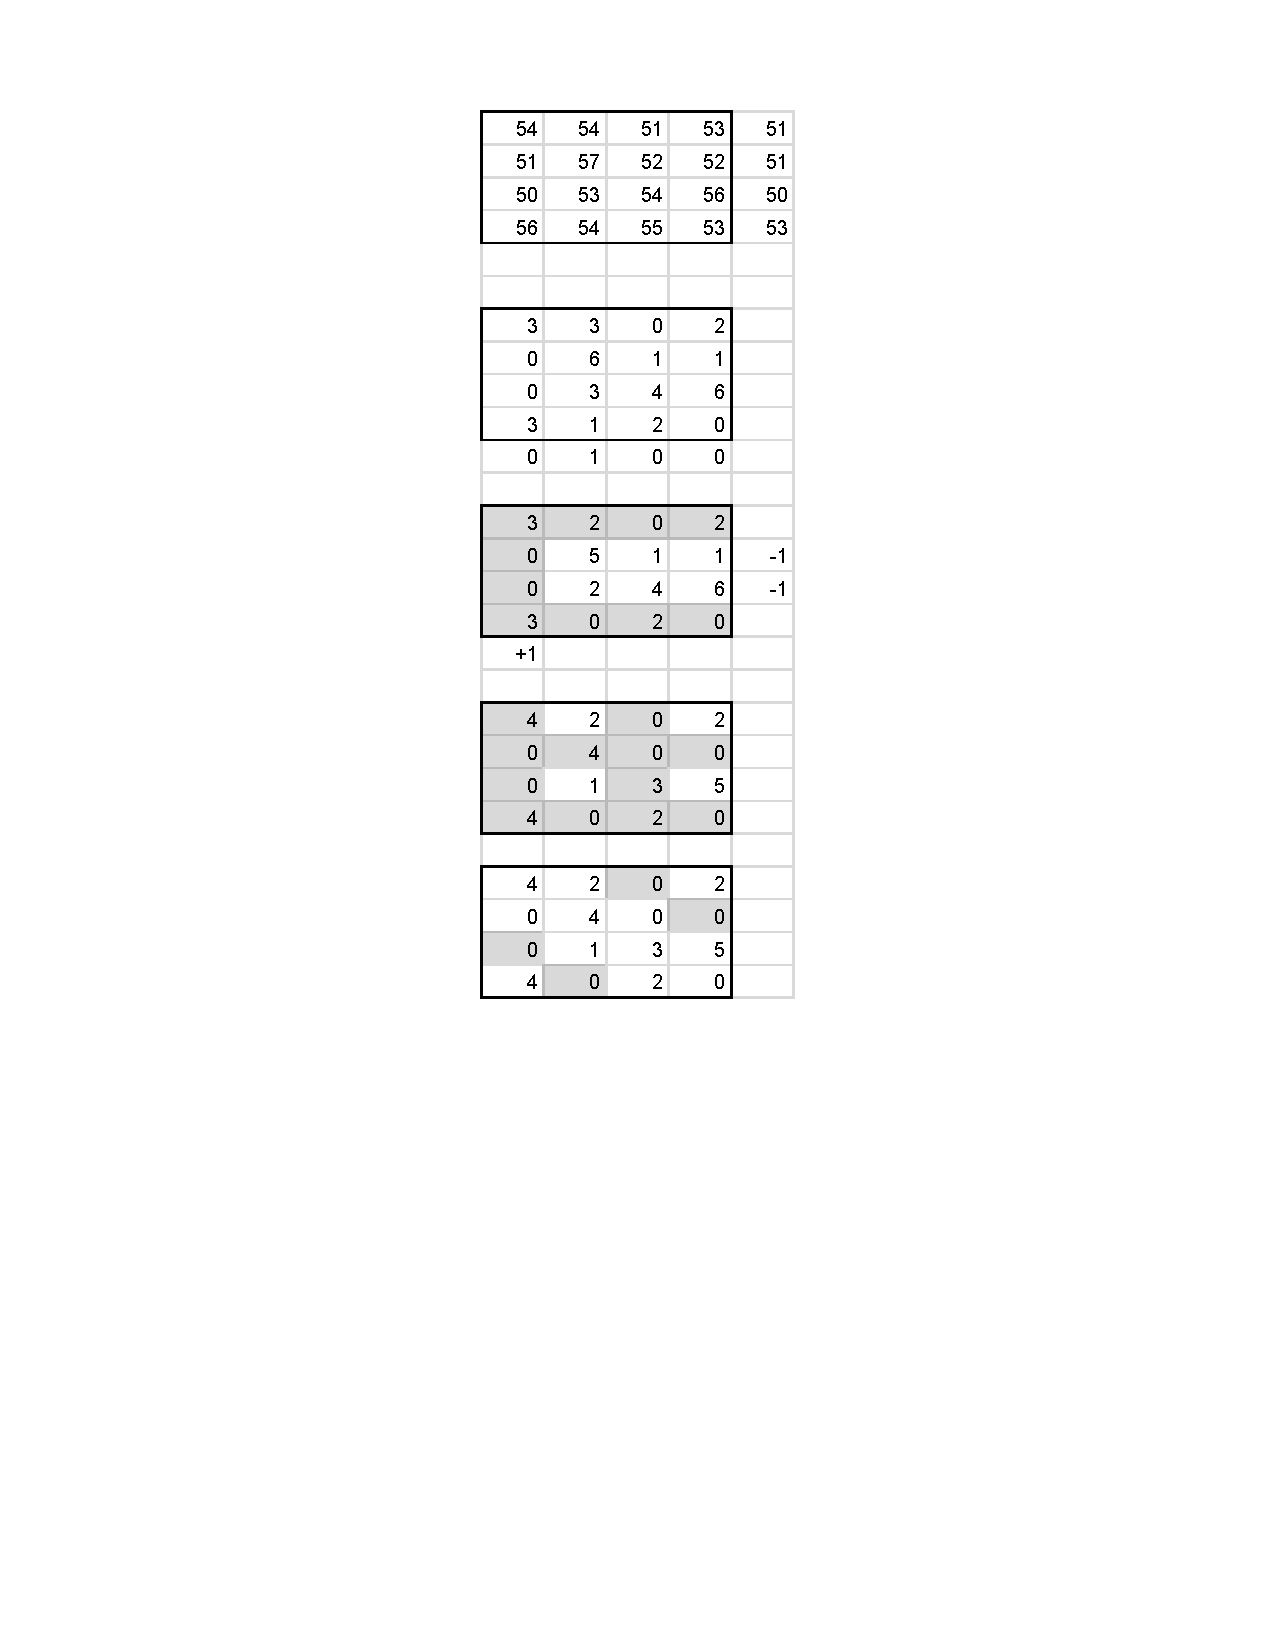
\includepdf[pages=-,pagecommand={},width=8.5in]{sheet2.pdf}

After the first iteration of subtracting minimums from rows and columns, the zero could be covered by a row/column cover of size $3 < n = 4$. Subtracting the minimum uncovered value from each uncovered row, and adding to the covered column, we then obtain a table whose zeros are covered by a row/column cover of at least size $4$. Making the only possible selection of row/column-independent zeros, we obtain the noted assignment. In the language of the problem, we have: Natalie to swim Fly, Brynn to swim Back, Angie to swim Free, Holly to swim Breast. And adding up the times for their respective strokes, we find a total time of $207$ seconds, which is optimal.

\end{document}